\chapter{Deep Learning and neural networks}

This chapter presents the basic concepts of deep learning and neural networks as well as how they can be used in reinforcement learning .


\section{Definition}

A neural network or NN \nomenclature{NN}{Neural Network} is a function that takes a tensor (a multi-dimensional vector) as input and then computes an output, which is another tensor of values. This computation involves a lot of parameters that are used to compute the output from the input. It can be noted as follows:

\begin{equation} \label{eq:NN simple}
    \mathbf{Y} = NN(\mathbf{X}; \pmb{\theta} )
\end{equation}


where $\mathbf{X}$ and $\mathbf{Y}$ are respectively the input and output tensors, $NN$ the neural network function and $\pmb{\theta}$ the neural network parameters.\\

The parameters of a neural network can be tuned or "learned" in such a way that the neural network approximates any given function. The parameters are learned using some data composed of some inputs and the outputs that we want our neural network to produce when fed with those inputs. 

For instance, if we want our neural network to be able to make the distinction between an apple and a banana, we will give him some data with photographs of apples and bananas (the inputs) as well as the corresponding labels for each photograph (the outputs). The network will then learn from this data by tuning its parameters. Then, the neural network should be able to classify some new images of apples and bananas that he has never been presented with during its training. In this example, the input tensors of the network are the values of all the pixels in the image, and the output will only have two values: the probability that the network thinks the input is a picture of an apple and the probability that it thinks it is a banana.\\

Other examples are:
\begin{itemize}
    \item Image up-scaling (resolution increase)
    \item Machine translation
    \item Image generation 
    \item Approximation of the Q-values in function of an agent's observation (see section \ref{sec:DRL})
\end{itemize}

\section{Working principle}

\subsection{A single neuron}

The basic building block of an artificial neural network is the artificial neuron. The name comes from the real neurons in our brains, because the technology has been inspired by it. Figure \ref{fig:neuron} shows a schematic view of a biological and an artificial neuron. An artificial neuron is a mathematical function that takes several values as input an computes one output. The output is a weighted sum of the inputs to which is also added a fixed value, called the bias. For a n inputs neuron, the output $y$ is thus calculated as follows:

\begin{equation} 
    y = b + \sum_{i=1}^n w_i x_i
\end{equation}
where $x_i$ is the i-th input, $w_i$ its corresponding weight and $b$ the neuron's bias. This can also be written in matrix form:

\begin{equation}  \label{eq:neuron}
    y = b + WX 
\end{equation}
where $W$ is a horizontal vector containing all the weights and $X$ is a vertical vector containing all the inputs.\\

\begin{figure}[h!]
    \centering
    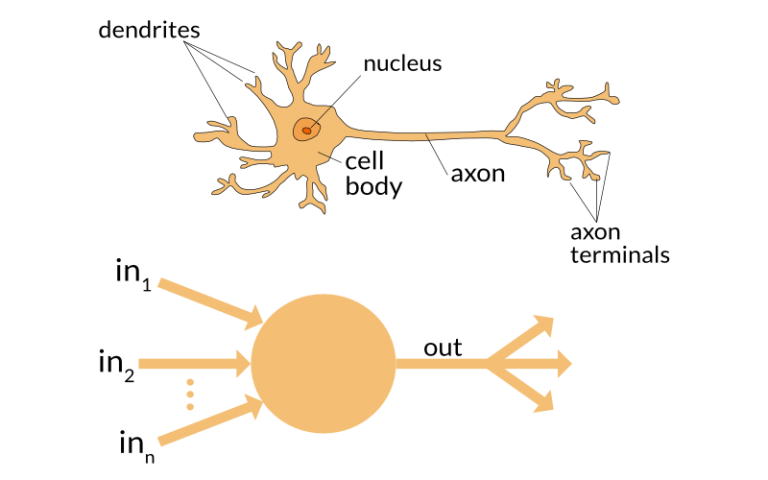
\includegraphics[width=.6\textwidth]{images/neuron.png}
    \caption{Schematic view of a biological and an artificial neuron \cite{neuron}}
    \label{fig:neuron}
\end{figure}

\subsection{Multiple neurons in a layer}

Furthermore, to obtain several outputs, several neurons can be stacked an form what is called a layer. Figure \ref{fig:neurons layer}\footnote{Figure generated with NN-SVG \cite{nnsvg}} shows a two neurons layer with five inputs. The output of such a neurons layer may be calculated as follows: 

\begin{equation} \label{eq:layer}
    Y = \textbf{W}X + B
\end{equation}

This is almost the same as (\ref{eq:neuron}), but now we have $Y$ a vertical vector containing all outputs, $B$ a vertical vector containing the biases of every neuron and $\textbf{W}$ a two-dimensional matrix containing every weight of every neuron, that is, all the $W$ horizontal vectors from (\ref{eq:neuron}) of all the neurons, stacked on top of each other. 

\begin{figure}[h!]
    \centering
    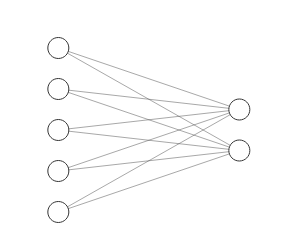
\includegraphics[width=.6\textwidth]{images/neuron layer}
    \caption{Schematic view of a two neurons layer with five inputs}
    \label{fig:neurons layer}
\end{figure}

\subsection{Approximating nonlinear functions}

Earlier in this chapter, we said that the aim of a neural network is to approximate a given function. However, (\ref{eq:layer}) clearly shows that the transformation between output and output is linear. Thus, only linear functions may be approximated, which is very limiting. To overcome this problem, some non-linearity is added into the neural networks. This is done by applying a non-linear function to the output of each neuron. In the field of deep learning, those functions are called activation functions. Figure \ref{fig:activation} shows four activation functions that are widely used in DL: sigmoid, Rectified Linear Unit (ReLU), hyperbolic tangent (tanh) and Exponential Linear Unit (ELU). Equations (\ref{eq:sigmoid}) to (\ref{eq:elu}) show the formula of those activation functions.

\begin{equation} \label{eq:sigmoid}
    sigmoid(x) = \frac{1}{(1-e^{-x}}
\end{equation}

\begin{equation} \label{eq:relu}
    ReLU(x) = max(0,x) = 
            \begin{cases}
                0 & \text{if $x<0$} \\
                x & \text{otherwise} 
            \end{cases}
\end{equation}

\begin{equation} \label{eq:tanh}
    tanh(x) = \frac{e^x-e^{-x}}{e^x+e^{-x}}
\end{equation}

\begin{equation} \label{eq:elu}
    ELU(x) = 
    \begin{cases}
        e^x-1 & \text{if $x<0$}\\
        x & \text{otherwise}
    \end{cases}
\end{equation}

\begin{figure}[h!]
    \centering
    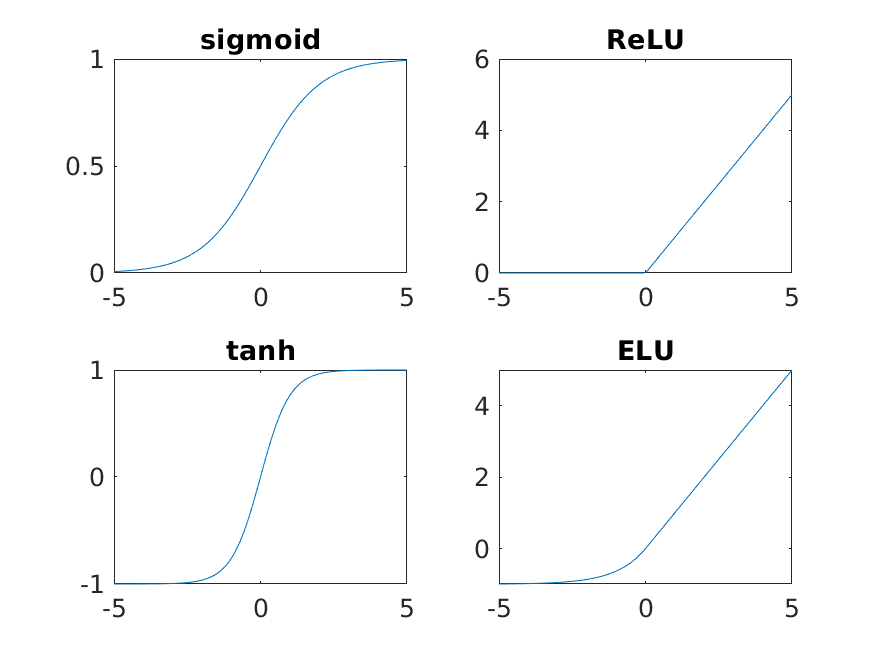
\includegraphics[width=.7\textwidth]{images/activation functions.png}
    \caption{Widely used activation functions}
    \label{fig:activation}
\end{figure}

\subsection{Deep neural networks}

In order to approximate more complex functions, deep neural networks are often used. They consist of several neurons layers stacked horizontally, where the output of each layer is fed as input to the next layer. Of course, a non-linear function is applied at the output of every layer. Figure \ref{fig:3 layers}\footnote{Figure generated with NN-SVG \cite{nnsvg}} shows a neural network with five inputs and two outputs. The data goes through three layers of 10 neurons before (called hidden layers). The output of the last hidden layer is fed as input to the output layer. The activation function is not shown on the figure, because it is considered to be part of each neuron, i.e. each neuron performs (\ref{eq:neuron}) then applies an activation function. 

\begin{figure}[h!]
    \centering
    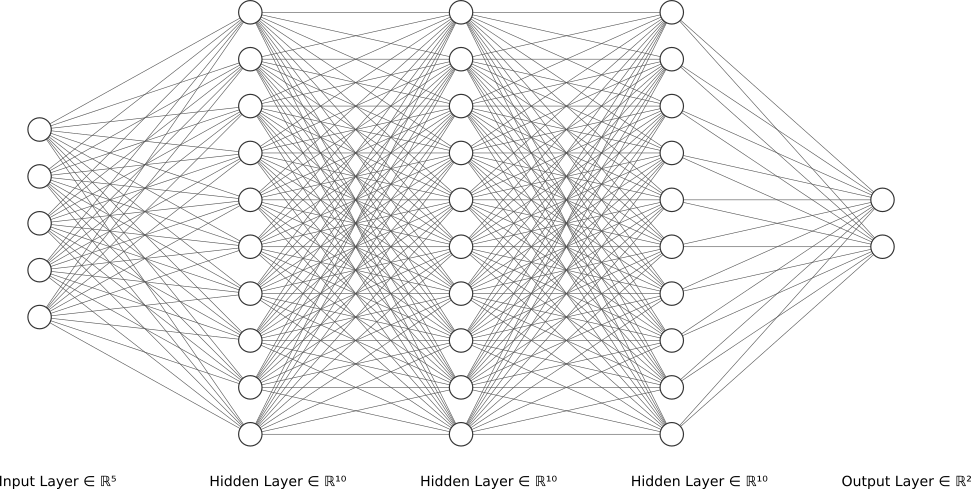
\includegraphics[width=.9\textwidth]{images/multi layers.png}
    \caption{Deep neural network}
    \label{fig:3 layers}
\end{figure}

\subsection{Supervised Learning}

In a neural network, the parameters ($\pmb{\theta}$ in equation \ref{eq:NN simple}) are the weights and biases of all the neurons in the network. Learning the weights and biases using a database composed of both inputs and their corresponding outputs is called supervised learning. This is opposed to another field in machine learning called unsupervised learning, where the training data is only composed of inputs. The objective is then to detect patterns in the data and classify it into categories.\\

\subsubsection{Loss function}

In supervised learning, the parameters are optimized by minimizing a cost function $J(\pmb{\theta})$ \nomenclature{$J(\pmb{\theta})$}{cost function}:

\begin{equation} \label{eq:loss}
    J(\pmb{\theta}) = L(\hat{Y},Y)
\end{equation}

where $\hat{Y} = NN(X;\pmb{\theta})$ and $L(\hat{Y},Y)$ is call the loss function and quantifies the difference between the expected output from the learning data and the output produced by the neural network. $\hat{Y}$ is often called the prediction and $Y$ the target.\\

A lot of different loss functions are used in Deep Learning, depending on the application. (\ref{eq:bce}) shows the Binary Cross Entropy (BCE) loss, which is used a lot when the outputs of the networks should be either 0 or 1. (\ref{eq:mse}) shows the Mean Square Error (MSE) loss. \\

% \begin{equation} \label{eq:l1 loss}
%     l_{L1}(\hat{Y}_i,Y_i) = \left|\hat{Y}_i - Y_i \right|
% \end{equation}

\begin{equation} \label{eq:bce}
    l_{BCE}(\hat{Y},Y) = \frac{1}{N} \sum_{i=1}^N Y_i\, ln(\hat{Y}_i) + (1-Y_i)ln(1-\hat{Y}_i)
\end{equation}

\begin{equation} \label{eq:mse}
    l_{MSE}(\hat{Y},Y) = \frac{1}{N} \sum_{i=1}^N \left(\hat{Y}_i - Y_i \right)^2
\end{equation}

This cost is rather easy to compute for given parameters and training data. However, it might be really heavy computation wise for big neural networks and/or data sets. Furthermore, this can be parallelized a lot and the computation time can be reduced very significantly by making this computation on GPUs (Graphics Processing Units), which have a very large number of cores that can work in parallel (up to tens of thousands) whereas classical CPUs (Central Processing Units) have at most a couple of tens of cores.\\

\subsubsection{Gradient descent}

The way this cost function is minimized is by applying the gradient descent algorithm, which is an iterative method. $\pmb{\theta}_t$ will thus denote the value of $\pmb{\theta}$ at iteration $t$. \\

First, the gradient of $J$ with respect to $\pmb{\theta}$ (i.e. $\nabla_{\pmb{\theta}} J$) is calculated. This is done using the backpropagation algorithm. The explanation of its working is out of the scope of this thesis.\\

Then, a small step in the negative direction of the gradient is taken, that is:
\begin{equation} \label{eq:backprop}
    \pmb{\theta}_{t+1} = \pmb{\theta}_t - \alpha \nabla_{\pmb{\theta}} J
\end{equation}

where $\alpha$ is called the learning rate. The discussion about this learning rate in RL (section \ref{sec:Q-learning}) is also valid here.\\

Those two steps are repeated until some stop criterion is achieved (Number of iterations, threshold value for the loss, accuracy of the predictions, ...). \\

Furthermore, the gradient is almost never calculated based on one single sample. Instead, the average over several (or all of the) samples of the training data is used. This sample is called a batch. The batch size is a very important hyperparameter in neural network training. A higher batch size often results in faster convergence and better results. However, beyond a certain point, increasing the batch size even more won't hardly increase the performance, but will increase the computation time.\\

Using only on or a few sample from the training data is called stochastic gradient descent (SGD). The computation time for one step in much smaller than for much bigger batches, but the direction of the steps is not optimal. Hence, with SGD, much more smaller steps are taken instead of bigger, but slower steps.\\

Such a method that calculates the size and direction of the steps to take at every iteration is called an optimizer.

\subsubsection{Momentum}

Other optimizers than the gradient descent exist. In order to increase the efficiency, a momentum term might be added. The momentum term takes into account the direction of the previous steps to determine the size and direction of the current step. It works as follows:

\begin{align} \label{eq:momentum}
    m_{t+1} &= \alpha\, \nabla_{\pmb{\theta}} J + \mu\, m_t\\
     \pmb{\theta}_{t+1} &= \pmb{\theta}_t - m_{t+1}
\end{align}
where $\mu$ is a parameter that determines how much the previous steps influence the current one.\\

An illustration of momentum applied to a two parameters optimization problem is show on figure \ref{fig:momentum}. The image can be visualize as a plane where the position represents the value of the two parameters. The black elliptical curves are iso-loss curves and the red dot is the optimal values of the two parameters for a minimal loss.\\

\begin{figure}[h!]
    \centering
    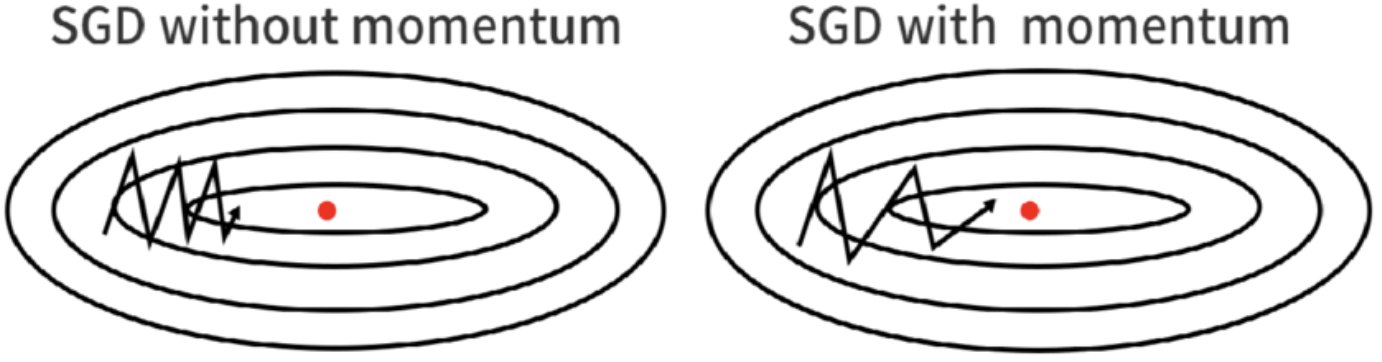
\includegraphics[width=.7\textwidth]{images/momentum.png}
    \caption{Stochastic Gradient Descent with and without momentum \cite{momentum}}
    \label{fig:momentum}
\end{figure}

\subsubsection{Other optimizers}

Other more sophisticated optimizers have been developed in the field of Deep Learning. The goal of every optimizer is to achieve faster convergence and/or to convergence towards better results (lower loss values). Adam \cite{adam} is maybe the most widely used optimizer in Deep Learning. It estimates the first and second momentum and computes several adaptive learning rates. 

\section{Recurrent neural networks}

\section{Deep Reinforcement Learning} \label{sec:DRL}


